%
% hilbertraum.tex
%
% (c) 2019 Prof Dr Andreas Müller, Hochschule Rapperswil
%
\section{Hilbertraum
\label{section:hilbertraum}}
\rhead{Hilbertraum}
Die bisher entwickelte Theorie ist aus zwei Gründen nicht ausreichend für das,
was wir vorhaben.

Ein endlichdimensionaler Vektorraum ist sicher ein geeigneter Rahmen zur
Beschreibung eines Signals, welches an endlich vielen Stellen abgetastet
wurde.
Für kontinuierliche Signale, also Funktionen $x(t)$,  reicht er aber nicht.
Zunächst ist die Menge aller Funktionen zwar ein Vektorraum, aber es ist
aussichtslos, eine endliche orthonrmierte Basis zu finden.
Vielmehr werden wir sehen, dass bereits der Raum der stetigen Funktionen
auf einem Interval unendlich viele Funktionen enthält, die in einem noch
zu definierenden Sinn aufeinander senkrecht stehen.
Wir müssen daher den Begriff erweitern, so dass auch unendlichdimensionale
Vektorräume behandelt werden können.

In der Praxis tauchen nicht nur Signale mit rellen Werten auf, sondern
auch solche mit komplexen Werten.
An entscheidenden Stellen im vorangegangen Abschnitt, insbesondere bei
der Konstruktion der Norm, haben wir verwendet,
dass $0 \le x^2$ ist für $x\in\mathbb R$. Für $x\in\mathbb C$ ist dies
nicht mehr wahr.
Der bisher formulierte Begriff des Skalarproduktes funktioniert daher
nicht für komplexe Signale.

Damit die endlichdimensionale Theorie vollständig übertragen werden kann,
müssen folgende Eigenschaften gerettet werden:
\begin{itemize}
\item {\bf Lineare Operationen:}
Signale können verstärkt (mit reellen Zahlen multipliziert) und überlagert
(addiert) werden.
Die Verallgemeinerung muss also die üblichen Rechenregeln bewahren,
sie muss also wieder ein Vektorraum sein.
Da es keine endlichdimensionale Basis mehr gibt, muss man unendlichen
Linearkombinationen einen Sinn geben können, was nur mit Hilfe des
Begriffs der Konvergenz von Folgen möglich ist.
Dazu wiederum muss man den Unterschied zwischen Vektoren messen können.
Vektorraum und Skalarprodukt werden in
Abschnitt~\ref{subsubsection:komplexevr-mit-skalarprodukt}
axomiatisch dargestellt.
\item {\bf Skalarprodukt:}
Das Skalarprodukt ist das Mass für die Ähnlichkeit zweier Funktionen
und gleichzeitig die Quelle eines Norm-Begriffs.
Abschnitt~\ref{subsection:norm-und-grenzwert} behandelt den Grenzwertbegriff.
\item {\bf Basis:}
Anstelle einer Basis genügt es orthonormierte Vektormengen zu finden,
mit denen sich jeder beliebige Vektor im Grenzwert linear kombinieren
lässt.
Abschnitt~\ref{subsection:hilbertraum-basis} erklärt den Begriff der
Hilbertraum-Basis.
\item {\bf Dualität:}
In einem endlichdimensionalen Vektorraum ist es so offensichtlich, dass
jede Linear-Form als Skalarprodukt mit einem geeigneten Vektor 
dargestellt werden kann.
Dies ermöglicht, einen Vektor als Linearform zu charakterisieren.
In einem unendlichdimensionalen Vektorraum ist dies nicht mehr
selbstverständlich.
Der Darstellungssatz von Riesz auf Seite~\pageref{subsubsection:riesz}
in Abschnitt~\ref{subsection:geometrie-hilbertraum}
stellt dies in einem Hilbertraum jedoch sicher.
\end{itemize}

\subsection{Komplexe Vektorräume mit Skalarprodukt
\label{subsubsection:komplexevr-mit-skalarprodukt}}
Es hindert uns nichts daran, in der Definition eines Vektorraums für die
Menge der Skalare auch komplexe Zahlen zuzulassen.
Ganz allgemein kann ein Vektorraum sinnvoll definiert werden, wenn die Menge
der Skalare ein sogenannter Körper ist, wenn also die Addition
und die Multiplikation mit von $0$ verschiedenen Skalaren umkehrbar sind.
Dies trifft natürlich für komplexe Zahlen zu, aber auch für $\mathbb Q$.

Im komplexen Vektorraum der komplexen Funktionen $C(\mathbb R,\mathbb C)$
lässt sich die besondere Rolle der Funktionen $t\mapsto e^{i\omega t}$ 
besser verstehen, auf denen die Fourier-Theorie basiert.

\begin{satz}
Die einzigen stetigen Funktionen, die Eigenvektoren von $T_b$ sind für
jeden beliebigen Wert von $b$ sind die Funktionen $t\mapsto e^{i\omega t}$.
\end{satz}

\begin{proof}[Beweis]
Sei $f$ eine Eigenfunktion aller Operatoren $T_b$ mit Eigenwert $\lambda(b)$.
$f$ kann keine Nullstelle haben.
Wäre nämlich $f(t_0)=0$, dann würde folgen
\[
(T_bf)(t_0) = f(t_0-b) = \lambda(b) f(t_0) = 0,
\]
die Funktion würde identisch verschwinden.

Mit $\lambda(b)$ sind aber alle Funktionswerte festgelegt, denn es 
gilt
\[
f(x) = f(0-(-x)) = T_{-x}f(0) = \lambda(-x) f(0).
\]
Die Funktion $\lambda$ ist bis auf eine Spiegelung eine Eigenfunktion.

Weiter kann man aus der Regel $T_{a+b}=T_aT_b$ schliessen, dass
\[
\lambda(a+b) f
=
T_{a+b}f
=
T_aT_bf
=
\lambda(a)\lambda(b)f
\]
sein muss, also  $\lambda(a+b)=\lambda(a)\lambda(b)$.
Die Exponentialfunktionen $t\mapsto e^{i\omega t}$ sind die einzigen
Funktionen, die als Lösung für $\lambda$ in Frage kommen.
\end{proof}

Die Definition der Länge eines Vektors und des Skalarproduktes auf dem
Vektorraum $\mathbb C^n$ erfordert etwas zusätzliche Aufmerksamkeit.
Die Quadratsumme der Komponenten funktioniert sicher nicht, da komplexe
Zahlen negative Quadrate haben können.
Die naheliegende Norm ist daher
\begin{equation}
\|v\| = \sum_{k=1}^n |v_k|^2.
\label{buch:hilbert:norm1}
\end{equation}
Sie ist für alle von $0$ verschiedenen Vektoren positiv, also positiv
definit.
Wir wollen diese Norm aber aus einem Skalarprodukt gewinnen.
Eine Möglichkeit ist
\begin{equation}
\langle u,v\rangle = \sum_{k=1}^n u_k\bar{v}_k.
\label{hilbert:skalaransatz}
\end{equation}
Die zugehörige Norm ist tatsächlich \eqref{buch:hilbert:norm1}.

Allerdings ist diese Bildung nicht mehr linear im zweiten Faktor.
Multipliziert man $v$ mit $\lambda$ erhält man
\[
\langle u,\lambda v\rangle
=
\sum_{k=1}^n u_k\bar{\lambda} \bar{v}_k
=
\bar{\lambda}\sum_{k=1}^n u_k\bar{v}_k
=
\bar{\lambda}\langle u,v\rangle.
\]
Man sagt, $\langle\;\,,\;\rangle$ ist {\em konjugiert linear} oder
{\em sesquilinear} im zweiten Argument.
\index{konjugiert linear}%
\index{sesquilinear}%
Im ersten Argument ist $\langle\;\,,\;\rangle$ aber immer noch linear.

Die Konstruktion~\eqref{hilbert:skalaransatz} ist auch nicht mehr
symmetrisch, vielmehr gilt:
\[
\langle v,u\rangle
=
\sum_{k=1}^n v_k\bar{u}_k
=
\overline{\sum_{k=1}^n u_k\bar{v}_k}
=
\overline{\langle u,v\rangle}.
\]
Vertauschen der Faktoren führt zum konjugiert komplexen Wert des
Skalarproduktes.
Man nennt diese Symmetrieeigenschaft von $\langle\;\,,\;\rangle$
{\em hermitesch}.
Hermitesche Formen ermöglichen wieder eine Skalarproduktdefinition.
Das Skalarprodukt eines Vektors mit sich selbst ist nämlich
\[
\overline{\langle {\color{red}u},{\color{blue}u}\rangle}
=
\langle {\color{blue}u},{\color{red}u}\rangle.
\]
Nur die reellen Zahlen sind zu sich selbst konjugiert komplex, man kann
also schliessen, dass für eine hermitesche Form
$\langle u,u\rangle\in\mathbb R$ ist.

Dies führt uns auf die folgende Definition eines Skalarproduktes für einen
komplexen Vektorraum.
\index{Skalarprodukt, komplexes}%
\index{komplexes Skalarprodukt}%
\begin{definition}
Eine Funktion
\[
\langle\;\,,\;\rangle
\colon V\times V\to \mathbb C : (u,v) \mapsto \langle u,v\rangle
\]
heisst ein komplexes Skalarprodukt, wenn gilt:
\begin{enumerate}
\item $\langle \;\,,\;\rangle$ ist linear im ersten Argument.
\item $\langle \;\,,\;\rangle$ ist konjugiert linear im zweiten Argument.
\item $\langle\;\,,\;\rangle$ ist hermitesch,
d.~h.~$\langle u,v\rangle=\overline{\langle v,u\rangle}$.
\item $\langle \;\,,\;\rangle$ ist positiv definit, d.~h.~es gilt
$\langle u,u\rangle \ge 0$ mit Gleichheit nur falls $u=0$.
\end{enumerate}
\end{definition}

Die Herleitung der Cauchy-Schwarz-Ungleichung hat die Symmetrie
\index{Cauchy-Schwarz-Ungleichung}%
und die Bilinearität des Skalarproduktes verwendet, sie lässt sich
also auf diese hermitesche Skalarprodukt nicht direkt übertragen.
Wir rollen das Problem daher nochmals neu auf im Beweis des folgenden
Satzes.

\begin{satz}
Sei $V$ ein komplexer Vektorraum mit komplexem Skalarprodukt
$\langle\;\,,\;\rangle$,
dann gilt die Cauchy-Schwarz-Ungleichung
\[
|\langle u,v\rangle| \le \|u\|\cdot \|v\|
\]
mit Gleichheit genau dann, wenn $u$ und $v$ linear abhängig sind.
\end{satz}

\begin{proof}[Beweis]
Wie im reellen Fall berechnen wird die Norm von $u+tv$:
\begin{align*}
0&\le
\| u+tv\|=\langle u+tv,u+tv\rangle
=
\|u\|^2 + \bar{t}\langle u,v\rangle + t\langle v,u\rangle + |t|^2 \|v\|^2
\\
&=
\|u\|^2 + \bar{t}\langle u,v\rangle + t\overline{\langle u,v\rangle} + |t|^2 \|v\|^2
\end{align*}
mit Gleichheit genau dann, wenn $u+tv=0$.
Die mittleren beiden Terme enthalten das Skalarprodukt, durch die Wahl
$t=-\langle u,v\rangle/\|v\|^2$ wird daraus
\begin{align*}
0
&\le
\|u\|^2 - 2\frac{|\langle u,v\rangle|^2}{\|v\|^2}
+
\biggl(\frac{|\langle u,v\rangle|}{\|v\|^2}\biggr)^2\|v\|^2
\\
&=
\|u\|^2 - \frac{|\langle u,v\rangle|^2}{\|v\|^2}.
\end{align*}
Multiplikation mit $\|v\|^2$ liefert
\begin{align*}
0&\le \|u\|^2 \cdot \|v\|^2 - |\langle u,v\rangle|^2
\\
\Leftrightarrow
\qquad
|\langle u,v\rangle|^2
&\le \|u\|^2 \cdot \|v\|^2
\end{align*}
mit Gleichheit genau dann, wenn $u+tv=0$.
Damit ist die Cauchy-Schwarz-Ungleichung auch für den komplexen Fall bewiesen.
\end{proof}

Auch für ein komplexes Skalarprodukt gilt, dass die Werte der Norm
das Skalarprodukt eindeutig bestimmen.
Da die Norm jedoch immer reelle Werte annimmt, ist etwas mehr Arbeit
erforderlich, um den Imaginärteil des Skalarproduktes wiederzugewinnen.
Zunächst rechnen wir wie im Fall des reellen Skalarproduktes
\begin{align*}
\| u+v\|^2 
&=
\|u\|^2 + \langle u,v\rangle + \langle v,u\rangle + \|v\|^2
\\
&=
\|u\|^2 + \langle u,v\rangle + \overline{\langle u,v\rangle} + \|v\|^2
\\
&=
\|u\|^2 + 2\operatorname{Re}\langle u,v\rangle + \|v\|^2
\\
\Rightarrow\qquad
\operatorname{Re}\langle u,v\rangle
&=
\frac12(
\|u+v\|^2 - \|u\|^2 - \|v\|^2
).
\intertext{
Um den Imaginärteil zu bekommen, multiplizieren wir $v$ mit $i$:
}
\|u+iv\|^2
&=
\|u\|^2 + \langle u,iv\rangle + \langle iv,u\rangle + \|iv\|^2
\\
&=
\|u\|^2 -i \langle u,v\rangle + i\langle v,u\rangle + |i|^2 \|v\|^2
\\
&=
\|u\|^2 + \|v\|^2
-i (\langle u,v\rangle - \overline{\langle u,v\rangle})
\\
&=
\|u\|^2 + \|v\|^2
-i (2i\operatorname{Im}\langle u,v\rangle)
\\
&=
\|u\|^2 + \|v\|^2
+ 2\operatorname{Im}\langle u,v\rangle
\\
\Rightarrow\qquad
\operatorname{Im}\langle u,v\rangle
&=
\frac12(
\|u+iv\|^2- \|u\|^2 - \|v\|^2).
\end{align*}
Zusammengesetzt finden wir die Formel
\begin{equation}
\langle u,v\rangle
=
\frac12(
\|u+v\|^2 - \|u\|^2 - \|v\|^2
)
+
\frac{i}2(
\|u+iv\|^2- \|u\|^2 - \|v\|^2)
)
\label{hilbert:polarisierung}
\end{equation}
für das Skalarprodukt zweier beliebiger Vektoren, ausgedrückt
ausschliesslich mit der Norm.
Die Identität \eqref{hilbert:polarisierung} ist auch bekannt unter dem
Namen {\em Polar-Identität} oder {\em Polarisierung} des Skalarprodukts.
\index{Polar-Identität}%
\index{Polarisierung}%


\subsection{Norm und Grenzwert in einem Hilbertraum
\label{subsection:norm-und-grenzwert}}
Bis jetzt haben wir immer in endlichdimensionalen Vektorräumen gearbeitet.
Der tiefere Grund dafür war, dass die Arbeit mit unendlich vielen Basisvektoren
$e_k$, $k\in\mathbb N$, erfordert, dass Ausdrücken der Form
\begin{equation}
\sum_{k=1}^\infty a_k e_k
\label{hilbert:summe}
\end{equation}
einen Sinn gegeben werden muss.
Die Algebra definiert nur endliche Summen.
Eine unendliche Summe ist in einem rein algebraischen Kontext daher
sinnlos.
Ein Ausdruck wie \eqref{hilbert:summe} kann daher nur im Sinne eines
Grenzwertes verstanden werden.
In einem Vektorraum ist aber a priori nicht definiert, wie man die
Approximation eines Vektors $v$ durch eine Folge von Vektoren $v_k$ zu
verstehen hat.
Mit der Einführung des Skalarproduktes und der daraus abgeleiteten Norm
ändert sich das.
\begin{definition}
Sei $V$ ein Vektorraum mit Skalarprodukt.
Eine Folge $v_k\in V$ konvergiert gegen den Vektor $v\in V$ für $k\to\infty$,
wenn
\[
\| v_k - v\| \to  0 
\qquad\Leftrightarrow\qquad
\lim_{k\to\infty} v_k = v.
\]
\end{definition}

Man erwartet, dass eine Folge einen Grenzwert hat, wenn die Folgenglieder
immer näher zu\-ei\-nan\-der rücken.
\index{Grenzwert}%

\begin{definition}
Eine Folge $v_k\in V$ heisst {\em Cauchy-Folge}, wenn es für jedes
\index{Cauchy-Folge}%
$\varepsilon > 0$ ein $N(\varepsilon)\in\mathbb N$ gibt, so dass
$\|v_k - v_m\| < \varepsilon$ sobald $k,m>N(\varepsilon)$.
\end{definition}

Leider ist nicht garantiert, dass in einem komplexen Vektorraum eine
Cauchy-Folge auch tatsächlich einen Grenzwert hat.

\begin{beispiel}
Wir betrachten den Vektorraum
\[
c_0 = \{ X=(x_0, x_1, \dots ,x_k,0,\dots)\,| x_i \in \mathbb C\}
\]
von Folgen, die nur endlich viele Terme haben, die von $0$ verschieden sind.
Wir können diesem Vektorraum ein komplexes Skalarprodukt verpassen, indem wir
\[
\langle X,Y\rangle
=
\sum_{k=1}^\infty x_k\bar{y}_k
\]
setzen.
Da in beiden Folgen nur endlich viele Terme von $0$ verschieden sind, ist
die Summe auf der rechten Seite eine endliche Summe.
Ganz offensichtlich ist dies ein komplexer Vektorraum mit Skalarprodukt.
Jetzt betrachten wir die Folge
\begin{align*}
X_1 &= (1,0,0,0,\dots)
\\
X_2 &= \textstyle (1,\frac12,0,0,\dots)
\\
X_3 &= \textstyle (1,\frac12,\frac13,0,\dots)
\\
&\vdots
\\
X_k &= \textstyle (1,\frac12,\frac13,\dots,\frac1k,0,\dots)
\\
&\vdots
\end{align*}
Wir behaupten, dies sei ein Cauchy-Folge.
Dazu müssen wir Differentzen $\| X_n-X_m\|$ untersuchen.
Wir dürfen annehmen, dass $m < n$ ist.
Dann ist
\begin{equation}
\| X_n - X_m\|^2 = \sum_{k=m+1}^n \frac{1}{k^2}.
<
\sum_{k=m+1}^\infty \frac{1}{k^2}.
\label{hilbert:eulercauchy}
\end{equation}
Auf der rechten Seite steht ein Reststück der Reihe
\[
\sum_{k=1}^\infty \frac{1}{k^2},
\]
die Euler als Erster berechnet hat.
\index{Euler, Leonhard}%
Er hat den Wert $\frac{\pi^2}{6}$ gefunden.
Die Tatsache, dass die Reihe konvergiert, heisst aber auch, dass
es für jedes $\varepsilon >0$ eine Zahl $N(\varepsilon)$ gibt derart,
dass die rechte Seite von \eqref{hilbert:eulercauchy} kleiner ist
als $\varepsilon$, wenn nur $m,n>N(\varepsilon)$.
Die Folge $(X_k)$ ist also tatsächlich ein Cauchy-Folge.

Als Grenzwert kommt nur die Folge 
\[
X = \textstyle (1,\frac12, \frac13,\frac14,\dots)
\]
in Frage.
Und tatsächlich ist
\begin{equation}
\|X-X_n\|^2
=
\sum_{k=n+1}^\infty \frac1{k^2},
\label{hilbert:falscherabstand}
\end{equation}
wieder ein Reststück der Reihe von Euler, welches daher beliebig klein
gemacht werden kann.
Also konvergiert tatsächlich $X_k$ gegen $X$.

Die Folge $X$ ist aber gar nicht in $c_0$,
da alle Folgenglieder von $0$ verschieden sind.
Der Grenzwert einer Folge in $c_0$ muss also nicht mehr in $c_0$ sein.

Genau genommen haben wir schon in \eqref{hilbert:falscherabstand}
gemogelt.
Die Abstandsmessung in $c_0$ ist ja mit Hilfe einer endlichen Summe
definiert, hier haben wir aber eine unendliche Summe.
\end{beispiel}

Die Rekonstruktion eines Vektors mit Hilfe einer Linearkombination von
Basisvektoren kann also grundsätzlich nur dann funktionieren, wenn verlangt
wird, dass es zu jeder Cauchy-Folge von Vektoren auch tatsächlich einen
Grenzwert gibt.

\begin{definition}
Ein komplexer Vektorraum $V$ mit Skalarprodukt heisst {\em vollständig}, 
wenn jede Cauchy-Folge von Vektoren in $V$ einen Grenzwert in $V$ hat.
Ein solcher Vektorraum heisst {\em Hilbertraum}.
\end{definition}
\index{vollständig}%
\index{Hilbertraum}%

Der Vektorraum $c_0$ des obigen Beispiels lässt sich leicht zu einem
Hilbertraum machen.

\begin{beispiel}
Sei $l^2$ der komplexe Vektorraum der quadratsummierbaren komplexen
Zahlfolgen $(x_k)$, d.~h.
\index{$l^2$, Hilbertraum der quadratintegrierbaren Folgen}%
\[
l^2 = \left\{ (x_k)\,\left| \sum_{k=1}^\infty |x_k|^2 < \infty \right.\right\}
\]
mit dem Skalarprodukt
\[
\langle X,Y\rangle = \sum_{k=1}^\infty x_k\bar{y}_k.
\]
Die aus dem Skalarprodukt abgeleitete $l^2$-Norm ist
\[
\|x\|^2 = \sum_{k=1}^\infty |x_k|^2.
\]
Eine Cauchy-Folge $x^{(n)}\in l^2$ konvergiert gegen die Folge
\[
x_k = \lim_{n\to\infty} x_k^{(n)},
\]
da jedes einzelne Folgenglied in den Folgen $x^{(n)}$ eine Cauchy-Folge
bilden muss.
Daher ist $l^2$ ein Hilbertraum, er ist die naheligendste Verallgemeinerung
des komplexen Vektorraumes $\mathbb{C}^N$ mit Skalarprodukt auf unendlich
viele Dimensionen.
Da er auch relativ leicht verständlich ist und mit einem Computer gut
approximiert werden kann, wird er in den folgenden Kapiteln immer wieder
auftauchen.
\end{beispiel}

\subsection{Basis eines Hilbertraumes
\label{subsection:hilbertraum-basis}}
Eine Basis eines Vektorraums ist eine Menge von Vektoren, aus der sich
jeder beliebige Vektor linear kombinieren lässt.
In einem unendlichdimensionalen Vektorraum ist dieses Konzept nur
beschränkt nützlich, weil es von endlichen Summen ausgeht.

Das Skalarprodukt erlaubt auch in einem komplexen Hilbertraum den Begriff
der orthonormierten Basis zu definieren.
\index{orthonormierte Basis}
Eine Menge von orthonormierten Vektoren ist automatisch linear unabhängig.
In einem $n$-dimensionalen Vektorraum reicht das um sicherzustellen,
dass eine Menge von $n$ orthonormierten Vektoren eine Basis ist.
In einem undendlichdimensionalen Vektorraum reicht Orthonormalität
jedoch nicht um sicherzustellen, dass sich jeder Vektor beliebig genau
als Linearkombination approximieren lässt.

\begin{definition}
\label{geometrie:erzeugendensystem}
Eine Menge von Vektoren $\mathcal{B} = \{v_1,v_2,\dots\}\subset H$ in einem
Hilbertraum $H$ heisst eine {\em Erzeugendensystem}, wenn es keinen Vektor
\index{Erzeugendensystem}%
$v\in H$ gibt, der auf allen Vektoren von $\mathcal{B}$ senkrecht steht.
\end{definition}

Das folgende Beispiel zeigt, dass es eine einem unendlichdimensionalen
Vektorraum möglich ist, eine unendliche Folge orthonormierter Vektoren
und einen weiteren Vektor zu finden, der auf jedem Vektor senkrecht ist.

\begin{beispiel}
\label{geometrie:l2-beispiel}
\begin{figure}
\centering
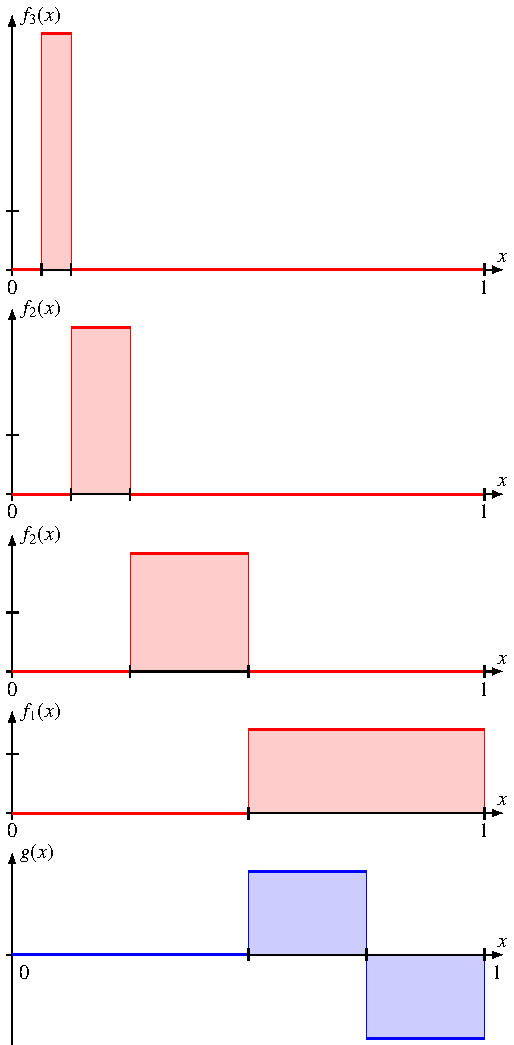
\includegraphics{chapters/1-geometrie/images/l2orth.pdf}
\caption{Familie von orthonormierten Funktionen $f_n(x)$, die alle auf der
Funktion $g(x)$ orthogonal sind.
Es gilt also $\langle f_n,f_m\rangle = \delta_{nm}$ und
$\langle f_n,g\rangle=0$.
\label{l2orth}}
\end{figure}
Wir zeigen Anhand eines Beispiels, dass der Vektorraum  der
quadrat-integrierbaren
Funktionen auf dem Interval $[0,1]$ mit einem Skalarprodukt
ausgestattet werden kann, welches ihn zu einem Hilbertraum macht.
Ausserdem konstruieren wir eine unendliche Menge von Funktionen, die alle
senkrecht aufeinander stehen.
Trotzdem werden wir einen weiteren Vektor finden, der auf all diesen
Vektoren senkrecht steht.

Als Erstes definieren wir das Skalarprodukt von Funktionen auf dem
Interval $[0,1]$ als
\[
\langle f, g\rangle
=
\int_0^1 f(x) \bar{g}(x)\,dx
\]
für Funktionen $f,g\colon [0,1]\to\mathbb C$.
Der Vektorraum der integrierbaren Funktionen mit diesem Skalarprodukt
heisst $L^2$ und wird in Kapitel~\ref{chapter:fourier} genauer untersucht.

Als nächstes konstruieren wir die Folge $f_i$ von Funktionen, die wie
folgt definiert sind:
\begin{align*}
f_1(x) &= \begin{cases}
\sqrt{2}&\qquad \frac12 \le x < 1\\
0\phantom{000}&\qquad\text{sonst}
\end{cases}
\\
f_2(x) &= \begin{cases}
2&\qquad \frac14 \le x < \frac12\\
0\phantom{000}&\qquad\text{sonst}
\end{cases}
\\
f_3(x) &= \begin{cases}
2^{\frac32}&\qquad \frac18 \le x < \frac14\\
0\phantom{000}&\qquad\text{sonst}
\end{cases}
\\
&\vdots
\\
f_n(x) &= \begin{cases}
2^{\frac{n}2}&\qquad \frac1{2^n} \le x < \frac2{2^n}\\
0\phantom{000}&\qquad\text{sonst,}
\end{cases}
\end{align*}
siehe auch Abbildung~\ref{l2orth}.
Die Funktion $f_n$ ist nur auf dem Interval $[2^{-n},2^{-n+1}]$ von
$0$ verschieden.
Zwei verschiedene Funktionen $f_n$ und $f_m$ mit $n\ne m$ sind also
nirgends gleichzeitig von $0$ verschieden, es folgt
$\langle f_n,f_m\rangle =0$.
Aber auch die Norm der Funktionen $f_n$ lässt sich leicht berechnen als
\[
\|f_n\|^2
=
\int_0^1 |f_n(x)|^2\,dx
=
\int_{2^{-n}}^{2^{-n+1}} (2^{\frac{n}2})^2 \,dx
=
\frac1{2^n}\cdot 2^n = 1.
\]
Somit ist gezeigt, dass die Funktionen $f_n$ orthonormiert im Sinne des
Skalarprodukts $\langle\;\,,\;\rangle$ sind.

Trotzdem gibt es eine Funktion $g$, die auf allen $f_n$ orthogonal ist.
Wir wählen
\[
g(x) = \begin{cases}
\sqrt{2}&\qquad \frac12 \le x < \frac34\\
-\sqrt{2}&\qquad \frac34 \le x < 1\\
0&\qquad\text{sonst.}
\end{cases}
\]
Diese Funktion ist ebenfalls normiert, denn es gilt
\[
\|g\|^2
=
\int_0^1 |g(x)|^2 \,dx
=
\int_{\frac12}^1 (\sqrt{2})^2\,dx
=
\frac12\cdot 2 = 1.
\]

Die Funktion $g$ ist nur auf dem Interval $[\frac12,1]$ von $0$ verschieden,
sie ist damit automatisch orthogonal auf allen Funktionen $f_n$ mit $n\ge 2$.
Für die Funktion $f_1$ ist
\[
\langle g,f_1\rangle
=
\int_0^1 g(x)\bar{f}_1(x)\,dx
=
\int_{\frac12}^1 g(x)\,dx
=
\int_{\frac12}^{\frac34}\sqrt{2}\,dx
+
\int_{\frac34}^1-\sqrt{2}\,dx
=
\frac14 \sqrt{2} - \frac14 \sqrt{2} = 0.
\]
Die Funktion $g$ ist also orthogonal auf allen Funktionen $f_n$.
In einem unendlichdimensionalen Hilbertraum kann es also selbst
neben einer unendlich grossen Menge von orthonormierten Vektoren 
noch einen weiteren Vektor geben, der senkrecht auf allen steht.
\end{beispiel}

Das Beispiel lässt sich beliebig erweitern: Jede Skalierung
$\tilde{D}_{2^n}g$ ist ebenfalls orthogonal auf allen Vektoren $f_k$.
Offenbar gibt die Folge $f_k$ den Hilbertraum nur sehr skelettartig wieder.

\begin{beispiel}
Wir betrachten den Hilbertraum $l^2$, dessen Vektoren Folgen
$a=(a_k)_{k\in\mathbb N}$ von komplexen Zahlen sind mit dem Skalarprodukt
\begin{equation}
\langle a,b\rangle = \sum_{k\in\mathbb N} a_k\bar{b}_k.
\label{l2:beispiel:erzeugendensystem}
\end{equation}
Die Vektoren $e^{(i)}$ mit den Komponenten
\[
e^{(i)}_k = \delta_{ik}
\]
sind überall $0$ ausser das Folgenglied mit der Nummer $i$, welches $1$
ist. 
Diese Vektoren haben Länge $1$ im Sinne des Skalarproduktes
\eqref{l2:beispiel:erzeugendensystem} und sie sind orthogonal:
\[
\langle e^{(i)}, e^{(j)}\rangle
=
\sum_{k\in\mathbb N} e^{(i)}_k\bar{e}^{(j)}_k
=
\sum_{k\in\mathbb N} \delta_{ik}\delta_{jk}
=
\delta_{ij}.
\]
Die Vektoren $e^{(i)}$ sind aber auch ein Erzeugendensystem, wie man sich
wie folgt überzeugen kann.
Gäbe es einen Vektor $v\in l^2$, dessen Skalarprodukt mit allen $e^{(i)}$
verschwindet, dann würde für alle $i$ folgen
\[
0
=
\langle v,e^{(i)}\rangle
=
\sum_{k\in\mathbb N} v_ke^{(i)}_k
=
\sum_{k\in\mathbb N} v_k\delta_{ik}
=
v_i,
\]
d.~h.~der Vektor $v$ ist $0$.
\end{beispiel}

Die naheliegende Erweiterung des Begriffs der orthonormierten Basis
eines endlichdimensionalen Vektorraums ist jetzt der Begriff der
Hilbertbasis.

\begin{definition}
Ein aus orthonormierten Vektoren bestehendes Erzeugendensystem
eines Hilbertraumes heisst {\em Hilberbasis}
\end{definition}
\index{Hilbertbasis}%

\begin{satz}
Wenn die Vektoren $\{e_k\,|\, 1\le k\le n\}$ eine Hilbertbasis des
Hilberraumes $H$ bilden,
dann lässt sich jeder Vektor $v\in H$ als Linearkombination
\[
v
=
\sum_{k=1}^\infty \hat{v}_k e_k
\]
der Vektoren $e_k$ schreiben.
Die Koeffizienten sind eindeutig bestimmt und können mit Hilfe des
Skalarproduktes als
\[
\hat{v}_k = \langle v,e_k\rangle
\]
gefunden werden.
Ausserdem gilt für das Skalarprodukt die Plancherel-Identität
\index{Plancherel-Identität}%
\begin{align*}
\langle u,v\rangle &= \sum_{k=1}^\infty \hat{u}_k\bar{\hat{v}}_k
\\
\| u \|^2 &= \sum_{k=1}^\infty |\hat{u}_k|^2.
\end{align*}
\end{satz}

Die Abbildung $T\colon V\to l^2: v\mapsto (\hat{v}_k\,|\,1\le k)$
ist also wie im reellen Fall eine {\em Isometrie} von Hilberträumen.
\index{Isometrie}%

\subsection{Geometrie des Hilbertraumes
\label{subsection:geometrie-hilbertraum}}
Das Skalarprodukt in einem endlichdimensionalen Vektorraum formalisiert
den Begriff der Orthogonalität, der die Grundlage für viele Aspekte
der geometrischen Anschauung ist.
Und tatsächlich zeigen die nachstehenden Entwicklungen dieses Abschnitts,
dass Aussagen wie die Existenz eines Orthogonalkomplements tatsächlich
auch in einem Hilbertraum Gültigkeit haben.
Dies bedeutet, dass wir uns bei Argumenten in einem Hilbertraum von 
der geometrischen Intuition leiten lassen können, solange wir nicht
von Eigenschaften Gebrauch machen, die von der endlichen Dimensionalität
des Anschauungsraumes abhängen.

\subsubsection{Formel von Pythagoras}
\index{Pythagoras-Formel}%
Die Pythagoras-Formel gilt auch für Vektoren in einem Hilbertraum.
Sind $x$ und $y$ orthogonale Vektoren in $H$, d.~h.~$x\perp y$, dann
gilt
\begin{equation}
\|y-x\|^2
=
\langle y-x,y-x\rangle
=
\|y\|^2
-
2\operatorname{Re}\underbrace{\langle y,x\rangle}_{\displaystyle=0}
+
\|x\|^2
=
\|x\|^2 + \|y\|^2.
\label{formel:pythagoras}
\end{equation}

\subsubsection{Parallelogrammregel}
\index{Parallelogrammregel}%
\begin{satz}
\label{satz:parallelogrammregel}
Seien $x,y\in H$ Vektoren in einem Hilbertraum, dann gilt
\begin{equation}
2\|x\|^2 + 2\|y\|^2
=
\| x+y\|^2 + \|x-y\|^2.
\label{formel:parallelogrammregel}
\end{equation}
Die Formel~\eqref{formel:parallelogrammregel} heisst die
{\em Parallelogrammregel}.
\end{satz}

\begin{proof}[Beweis]
Wir berechnen die Normquadrate auf der rechten Seite von 
\eqref{formel:parallelogrammregel} mit Hilfe des Skalarproduktes:
\begin{align*}
\|x+y\|^2 + \|x-y\|^2
&=
\langle x+y,x+y\rangle + \langle x-y,x-y\rangle
\\
&=
\|x\|^2 + \langle x,y\rangle + \langle y,x\rangle + \|y\|^2
+
\|x\|^2 - \langle x,y\rangle - \langle y,x\rangle + \|y\|^2
\\
&=
2\|x\|^2 + 2\|y\|^2.
\end{align*}
Dies ist linke Seite der Parallelogrammregel~\eqref{formel:parallelogrammregel}.
\end{proof}

\begin{figure}
\centering
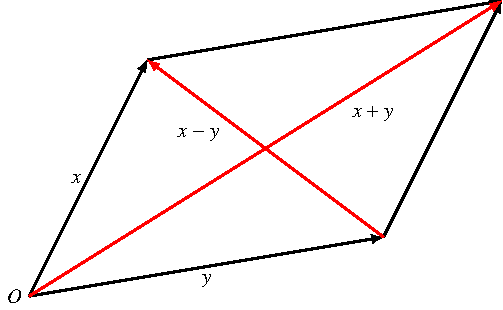
\includegraphics{chapters/1-geometrie/images/parallelogramm.pdf}
\caption{Parallelogramm-Regel (Satz~\ref{satz:parallelogrammregel})
\label{figure:parallelogrammregel}}
\end{figure}


Die Parallelogramm-Regel besagt, dass die Summe der Quadrate über den
Seiten eines Parallelgramms gleich der Summe der Quadrate über den
Diagonalen ist.
Dies ist in Abbildung~\ref{figure:parallelogrammregel} illustriert.

\subsubsection{Orthonormalisierung}
\index{Orthonormalisierung}%
Der Gram-Schmidt-Algorithmus zur Orthonormalisierung funktioniert auch
\index{Gram-Schmidt-Algorithmus}%
in einem Hilbertraum.

\begin{satz}
\label{satz:orthonormierung}
Sind $\{b_1,\dots,b_n\}\subset H$ eine endliche Menge von orthonormieren
Vektoren in $H$ und $a\in H$ ein Vektor, der nicht Linearkombination
der Vektoren $b_1,\dots,b_n$ ist.
Dann ist
\[
b
=
\frac{a-\langle a,b_1\rangle b_1-\dots-\langle a,b_n\rangle b_n}%
{|a-\langle a,b_1\rangle b_1-\dots-\langle a,b_n\rangle b_n|}
=
\frac{a-\displaystyle\sum_{k=1}^n \langle a,b_k\rangle b_k}%
{\biggl| a-\displaystyle\sum_{k=1}^n \langle a,b_k\rangle b_k\biggr|}
\]
ein Einheitsvektor, der zu allen $b_i$ orthogonal ist, insbesondere sind
die Vektoren
$b_1,\dots,b_n,b$ orthonormiert.
\end{satz}

\begin{proof}[Beweis]
Nach Definition ist $b$ ein Einheitsvektor
Das Skalarprodukt mit $b_i$ ist
\begin{align*}
\langle b, b_i\rangle
&=
\frac{\biggl\langle a-\displaystyle\sum_{k=1}^n \langle a,b_k\rangle b_k,b_i\biggr\rangle}%
{\biggl| a-\displaystyle\sum_{k=1}^n \langle a,b_k\rangle b_k\biggr|}
=
\frac{\langle a,b_i\rangle-\displaystyle\sum_{k=1}^n \langle a,b_k\rangle \langle b_k,b_i\rangle}%
{\biggl| a-\displaystyle\sum_{k=1}^n \langle a,b_k\rangle b_k\biggr|}
\\
&=
\frac{\langle a,b_i\rangle-\displaystyle\sum_{k=1}^n \langle a,b_k\rangle \delta_{ki}}%
{\biggl| a-\displaystyle\sum_{k=1}^n \langle a,b_k\rangle b_k\biggr|}
=
\frac{\langle a,b_i\rangle-\langle a,b_i\rangle}%
{\biggl| a-\displaystyle\sum_{k=1}^n \langle a,b_k\rangle b_k\biggr|}
=0,
\end{align*}
also ist $b$ orthogonal zu $b_i$ für alle $i=1,\dots,n$.
\end{proof}

Daraus lässt sich ableiten, dass jede endliche Menge von linear unabhängigen
Vektoren in einem Hilbertraum in eine orthonormierte Menge von Vektoren
verwandelt werden kann.

\subsubsection{Abstand zu einer Geraden}
\index{Abstand zu einer Geraden}
\begin{figure}
\centering
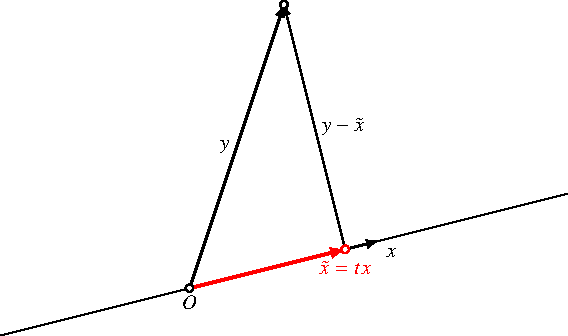
\includegraphics{chapters/1-geometrie/images/abstand.pdf}
\caption{Satz~\ref{satz:abstand} besagt, dass es zu einem Punkt $y$ ausserhalb
der Geraden $\{tx\;|\;t\in\mathbb C\}$ einen Punkte $\tilde{x}$ auf der
Geraden gibt, der minimalen Abstand von $y$ hat.
\label{figure:geradenabstand}}
\end{figure}
In einem reellen Vektorraum $H$ mit Skalarprodukt kann man zu einem Vektor
$y\in H$ und einem Richtungsvektor $x\in H$ immer einen Vektor
$\tilde{x}$ finden, der ein Vielfaches von $x$ ist und minimale Entfernung
von $y$ hat.
Das komplexe Skalarprodukt eines (komplexen) Hilbertraumes ermöglicht, 
das folgende analoge Minimalproblem zu lösten (Siehe auch
Abbildung~\ref{figure:geradenabstand}).

\begin{satz}
\label{satz:abstand}
Seien $y,x\in H$ gegeben, dann gibt es einen eindeutigen Vektor $\tilde x=tx$
derart, dass der Abstand
\[
\| y - \tilde{x}\|
=
\inf \{ \| y-t x\|\;|\; t \in \mathbb C\}
=:d
\]
zu $y$ minimal wird.
Ausserdem ist $y-\tilde{x}\perp x$.
\end{satz}

\begin{proof}[Beweis]
Der Abstand von $y$ zum Punkt $tx$ ist
\begin{align*}
\| y-tx \|^2
&=
\|y\|^2
-\langle y,tx\rangle
-\langle tx,y\rangle
+
|t|^2\|x\|^2
\notag
\\
&=
\|y\|^2
-\bar{t} \langle y,x\rangle
-t \langle x,y\rangle
+
|t|^2\|x\|^2
\notag
\\
&=
\|y\|^2
-2\operatorname{Re}(t\langle x,y\rangle)
+
|t|^2\|x\|^2.
\end{align*}
Der Abstand wird minimal, wenn der mittlere Term möglichst klein wird.
Dieser Fall tritt ein, wenn $t\langle x,y\rangle$ reell ist.

Schreibt man $t=\tau e^{i\varphi}$ mit $\tau\in\mathbb R$ derart, dass
$e^{i\varphi}\langle x,y\rangle=|\langle x,y\rangle|\in\mathbb R$,
dann folgt
\begin{equation}
\| y-tx \|^2
=
\|y\|^2
-2\tau|\langle x,y\rangle|
+
\tau^2\|x\|^2.
\label{min:minimalabstand}
\end{equation}
Mit Hilfe von $\tau$ und $\varphi$ kann man das Skalarprodukt auch
schreiben als $\langle x,y\rangle = e^{-i\varphi}|\langle x,y\rangle|$
oder $\langle y,x\rangle = e^{i\varphi}|\langle x,y\rangle|$.

Der Abstand~\eqref{min:minimalabstand} ist ein quadratischer Ausdruck
$a\tau^2 + b\tau +c$ der reellen Variablen $\tau$ mit
$a=\|x\|^2$, $b=-2|\langle x,y\rangle|$ und $c=\|y\|^2$.
Das Minimum wird für $t=-b/2a=|\langle x,y\rangle|/\|x\|^2$ erreicht.
Wir setzen daher
\[
\tilde{x}
=
tx
=
\tau e^{i\varphi}x
=
\frac{|\langle x,y\rangle|}{\|x\|^2}
e^{i\varphi}x.
\]
Das Skalarprodukt ist
\begin{align*}
\langle y-\tilde x,x\rangle
&=
\langle y,x\rangle - \tau e^{i\varphi}\langle x,x\rangle
=
e^{i\varphi}|\langle y,x\rangle|
- \frac{|\langle y,x\rangle|}{\|x\|^2} e^{i\varphi}\|x\|^2
=
0,
\end{align*}
was die behauptete Orthogonalität von $y-\tilde{x}$ und $x$ beweist.
\end{proof}

Der Satz besagt, dass es zu einem Vektor $y$ immer einen Punkt auf der 
komplexen Geraden $\{ tx\;|\; t\in\mathbb C\}$ gibt derart, dass der Abstand
minimal zu $y$ ist.

\begin{satz}
\label{satz:minimalallgemein}
Sei $x,y,z\in H$ mit $\|z\|\ne 0$ und sei $d$ der Abstand der (komplexen)
Geraden durch $x$ mit Richtungsvektor $z$ von $y$.
Dann gibt es einen Punkt $\tilde{x}$ auf der Geraden derart, dass
$d=\|y-\tilde{x}\|$ und $y-\tilde{x}\perp z$.
\end{satz}

\begin{proof}[Beweis]
Satz~\ref{satz:minimalallgemein} folgt aus Satz~\ref{satz:abstand}, indem
man für das $y$ in Satz~\ref{satz:abstand} den Vektor $y-x$ verwendet und
für das $x$ den Vektor $z$.
\end{proof}

\subsubsection{Approximationen des minimalen Abstands}
Sei $V$ ein Unterraum von $H$ und $y\in H$.
Der Abstand von $y$ von $V$ ist
\[
d = \inf \{ \| y - x\| \;|\; x \in V\}.
\]
In einem Hilbertraum ist es nicht mehr selbstverständlich, dass es auch
einen Vektor $x\in V$ gibt, der das Minimum realisiert, dass also
$ d = \|y-x\|$.
Wir können aber zeigen, dass gute Approximationen des minimalen Abstands
nicht weit voneinander entfernt sein können.

\begin{satz}
\label{satz:approx}
Sei $y\in H$ und $V$ ein Unterraum von $H$.
Sei $d=\inf \{ \|y-x\| \;|\;x\in V\}$ der Abstand von $y$ zum Unterraum $V$.
Sind $x_1,x_2$ zwei verschiedene Approxmationen des minimalen Abstands, d.~h.
\[
\| y-x_1\|^2 = d^2+\varepsilon_1
\qquad\text{und}\qquad
\| y-x_2\|^2 = d^2+\varepsilon_2
\]
In Abbildung~\ref{figure:approx} ist die Gerade $g$ durch die Punkte $x_1$
und $x_2$ dargestellt.
Dann ist 
\begin{equation}
\|x_1-x_2\| \le \sqrt{\mathstrut\varepsilon_1}+\sqrt{\mathstrut\varepsilon_2}.
\label{satz:approx:ungleichung}
\end{equation}
\end{satz}

\begin{figure}
\centering
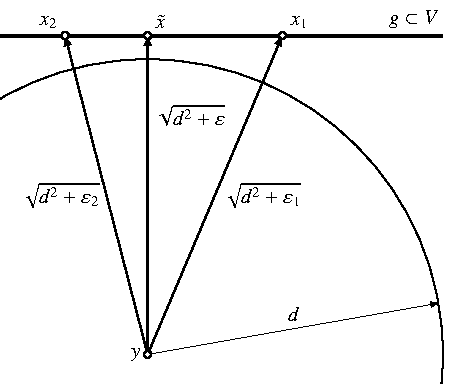
\includegraphics{chapters/1-geometrie/images/approx.pdf}
\caption{Approximation des minimalen Abstands des Punktes $y$ von
einer Geraden durch die Punkte $x_1$ und $x_2$.
Es lässt sich immer ein Punkt $\tilde{x}$ auf der Geraden $g$ durch
$x_1$ und $x_2$ finden, der eine noch bessere Approximation ist und so,
dass $y-\tilde{x}$ orthogonal ist zur Geraden.
Es folgt die Abschätzung~\eqref{satz:approx:ungleichung} für 
$\|x_1-x_2\|$ (Siehe auch Satz~\ref{satz:approx}).
\label{figure:approx}}
\end{figure}

\begin{proof}[Beweis]
Die beiden Vektoren $x_1$ und $x_2$ liegen auf der Geraden durch $x_1$ 
mit Richtungsvektor $z=x_2-x_1$.
Der minimale Abstand eines Punktes auf der Geraden durch $x_1$ mit 
Richtungsvektor $z$ ist mindestens $d$.
Wir schreiben ihn
\[
\inf \{ \|y- (x_1+tz)\|^2 \;|\; t\in \mathbb C\}
=
d^2 + \varepsilon.
\]
Nach dem Satz~\ref{satz:minimalallgemein} gibt es einen Vektor $\tilde{x}$
auf der Geraden durch $x_1$ mit Richtungsvektor $z$ derart, dass der minimale
Abstand durch $\tilde{x}$ realisiert wird, also
$\|y-\tilde{x}\|^2 = d^2+\varepsilon$.
Ausserdem ist $y-\tilde{x}\perp z$.

Da $y-\tilde{x}$ und $z$ orthogonal sind, kann man die Abstände
$\|y-x_i\|$ mit der Formel von Pythagoras \eqref{formel:pythagoras}
berechnen:
\begin{align*}
d^2 + \varepsilon_1
=
\|y-x_1\|^2 &= \|y-\tilde{x}\|^2 + \|\tilde{x}-x_1\|^2
=
\|\tilde{x}-x_1\|^2 + d^2 + \varepsilon
&&\Rightarrow&
\|\tilde{x}-x_1\|^2&=\varepsilon_1-\varepsilon
\\
d^2 + \varepsilon_2
=
\|y-x_2\|^2 &= \|y-\tilde{x}\|^2 + \|\tilde{x}-x_2\|^2
=
\|\tilde{x}-x_2\|^2 + d^2 + \varepsilon
&&\Rightarrow&
\|\tilde{x}-x_2\|^2&=\varepsilon_2-\varepsilon
\end{align*}
Damit kann man den Abstand zwischen $x_1$ und $x_2$ berechnen:
\[
\|x_1-x_2\|
\le
\|x_1-\tilde{x}\| + \| \tilde{x}-x_2\|
=
\sqrt{\mathstrut\varepsilon_1-\varepsilon}
+
\sqrt{\mathstrut\varepsilon_2-\varepsilon}
\le
\sqrt{\mathstrut\varepsilon_1} + \sqrt{\mathstrut\varepsilon_2}.
\]
Damit ist die Ungleichung \ref{satz:approx:ungleichung} bewiesen.
\end{proof}

\subsubsection{Orthogonalkomplement}
\index{Orthogonalkomplement}%
In einem endlichdimensionalen Vektorraum mit Skalarprodukt gibt es zu
einem abgeschlossenen Unterraum immer ein orthogonales Komplement,
selbst dann, wenn der Vektorraum nicht abgeschlossen ist.
Wenn man nämlich für den Unterraum eine endliche Basis wählt, ist das
Orthogonalkomplement charakterisiert durch endlich viele lineare 
Gleichungen, für die sich immer eine Lösungsmenge angeben lässt.
In einem unendlichdimensionalen Raum funktioniert dies nur noch, wenn
man Grenzwerte bestimmen kann, also zum Beispiel in einem Hilbertraum.

\begin{figure}
\centering
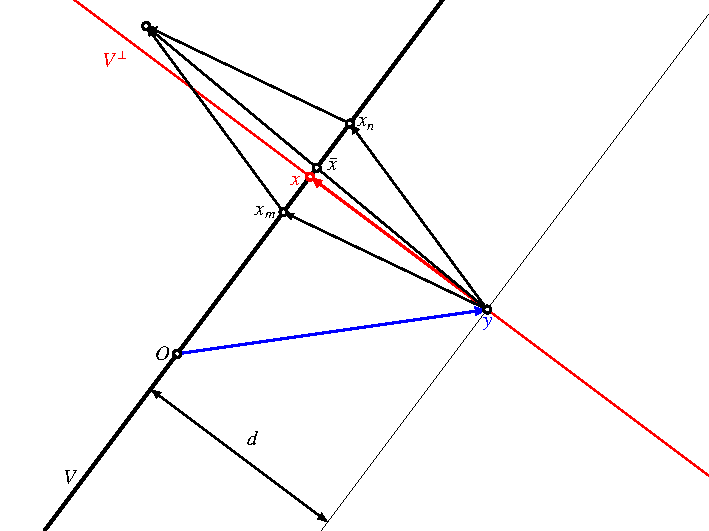
\includegraphics{chapters/1-geometrie/images/orthogonalkomplement.pdf}
\caption{Beweis der Existenz des Orthogonalkomplements in einem Hilbertraum
in Satz~\ref{satz:orthogonalkomplement}
\label{figure:orthogonalkomplement}}
\end{figure}

\begin{satz}
\label{satz:orthogonalkomplement}
Ist $V\subset H$ ein abgeschlossener Unterraum eines Hilbertraumes $H$,
lässt sich jeder Vektor $y\in H$ auf genau eine Art in $y = v+u$
zerlegen derart, dass $v \in V$ und $u\in V^{\perp}$,
d.~h.~$\langle z,u\rangle=0$ für alle $z\in V$.
\end{satz}

\begin{proof}[Beweis]
Sei $y\in H\setminus V$.
Die Funktion $v\mapsto \|y-v\|$ ist $\ge 0$, man kann also eine
Folge von Vektoren $v_k\in V$ finden, die den minimalen Abstand
approximieren, also derart, dass
\[
\lim_{k\to\infty} \|y-v_k\| = \inf_{v\in V} \|y-v\| =: d
\]
ist.
Dies ist gleichbedeutend damit, dass zu vorgegebenem $\varepsilon>0$ ein
$N$ gefunden werden kann, so dass $|d- \|y-v_k\|\,| < \varepsilon$ falls
$k>N$ ist (Siehe auch Abbildung~\ref{figure:orthogonalkomplement}).

Wir zeigen, dass $v_k$ eine Cauchy-Folge ist.
Dazu verwenden wir den Satz~\ref{satz:approx}, der besagt, dass zwei
gute Approximationen des minimalen Abstandes nicht weit voneinander
entfernt sein können.
Ist
$\|y-v_n\|^2 - d^2  < \varepsilon$ 
und
$\|y-v_m\|^2 - d^2  < \varepsilon$,
dann folgt nach Satz~\ref{satz:approx}, dass
\[
\|v_n-v_m\|
\le 2\sqrt{\mathstrut\varepsilon}
\qquad
\text{für $n,m>N.$}
\]
Da man $\varepsilon$ beliebig klein wählen kann, ist $(v_k)_{k\in\mathbb N}$
eine Cauchy-Folge.

Da $(v_k)_{k\in\mathbb N}$ eine Cauchy-Folge ist in $V$ und $V$ ausserdem
nach Voraussetzung abgeschlossen ist, folgt, dass $v_n$ gegen einen Grenzwert 
\[
v=\lim_{k\to\infty} v_k
\]
konvergiert.
$v$ ist der Vektor, für den das Minimum $\|y-u\|=d$ erreicht wird.
Auf diese Weise entsteht eine eindeutige Zerlegung $y = v + u$ mit $u=y-v$.

Es muss jetzt nur noch gezeigt werden, dass $u\in V^{\perp}$.
Dazu wenden wir den Satz~\ref{satz:minimalallgemein} auf die Gerade
durch $v$ mit einem beliebigen Vektor $z\in V$ an.
Da $v$ minimalen Abstand hat, ist $\tilde{v}=v$ und $z$ muss orthogonal
zu $y-v=u$ sein.
\end{proof}

\subsubsection{Darstellungssatz von Riesz
\label{subsubsection:riesz}}
\index{Satz von Riesz}%
\index{Darstellungssatz von Riesz}%
\index{Riesz, Friedrich}%
Zu einem gegebenen Vektor $v\in H$ eines Hilbertraums ist die Abbildung
\begin{equation}
H\to\mathbb C
:
u\mapsto \langle u,v\rangle
\label{hilbertraum:skalarproduktform}
\end{equation}
eine Linearform auf dem Vektorraum.
Linearformen auf einem endlichdimensionalen Vektorraum werden durch
einen Zeilenvektor beschrieben, es ist daher klar, dass es auch einen
Spaltenvektor gibt, mit dem sich die Linearform als Skalarprodukt
darstellen lässt.
In einem beliebigen unendlichdimensionalen Vektorraum ist der Vektorraum
der Linearformen typischerweise viel grösser.
Das besondere an Hilberträumen ist, dass sich jede stetige Linearform
als Skalarprodukt wie in \eqref{hilbertraum:skalarproduktform}
darstellen lässt.
Dies ist der Inhalt des Satzes von Riesz, der in diesem Abschnitt
bewiesen werden soll.

\begin{satz}[Riesz]
\label{geometrie:satz:riesz}
Ist $\varphi\colon H\to \mathbb C$ eine stetige Lineaform auf $H$, dann 
gibt es einen Vektor $v\in H$ derart, dass
\[
\varphi(u) = \langle u,v\rangle
\qquad
\forall u\in H.
\]
\end{satz}

\begin{proof}[Beweis]
Man betrachte den Raum
\[
V_1 = \{ u \in H \;|\;\varphi(u)=0\}.
\]
Da $\varphi$ eine stetige Linearform ist, ist $V_1$ ein abgeschlossener
Unterraum von $H$.
Falls $V_1=H$ folgt, dass $\varphi(u)=0$ für alle $u\in H$ ist,
also kann man $\varphi$ als Skalarprodukt mit dem Nullvektor schreiben:
$\varphi(u) = \langle u,0\rangle$.

Falls $V_1 \ne H$ ist, betrachtet man das orthogonale Komplement
\[
V_1^{\perp} = \{ v\in H\;|\; \langle v,u\rangle = 0\; \forall u\in V_1\},
\]
welches nach Satz~\ref{satz:orthogonalkomplement} existiert.
Angenommen, es gibt in $V_1^\perp$ zwei linear unabhängige Vektoren,
dann kann man diese orthonormalisieren.
Seien also $v'$ und $v''$ orthonormierte Vektoren in $V_1^\perp$.
Die Linearkombination
\[
v
=
\varphi(v'') v' - \varphi(v') v''
\in
V_1^\perp
\]
erfüllt $\varphi(v) = 0$, also ist $v\in V_1$.
Da die Zerlegung in $V_1$ und $V_1^\perp$ eindeutig ist, folgt
$v=0$.
Die Vektoren $v'$ und $v''$ waren also nicht linear unabhängig.
Es folgt, dass $V_1^\perp$ eindimensional ist.

Wir wählen einen beliebigen Vektor $v_0\in V_1^\perp$ und
setzen $v = \overline{\varphi(v_0)}v_0/\|v_0\|^2$.
Es gilt 
\[
\langle v_0,v\rangle
=
\biggl\langle v_0,
\overline{\varphi(v_0)}\frac{v_0}{\|v_0\|^2}
\biggr\rangle
=
\varphi(v_0).
\]
Ist $u$ ein beliebiger Vektor in $H$, dann lässt sich $u$ auf eindeutige
Weise schreiben als $u=u_1+u_2$ mit $u_1\in V_1$ und $u_2=\lambda $.
Es folgt
\begin{align*}
\varphi(u)
&=
\varphi(u_1) + \varphi(\lambda v_0)
=
\lambda \varphi(v_0)
\\
\langle u,v\rangle
&=
\langle u_1,v\rangle + \langle u_2,v\rangle
=
\lambda \underbrace{\langle v_0,v\rangle}_{\displaystyle=\varphi(v_0)}
=
\lambda \varphi(v_0).
\end{align*}
Es ist also tatsächlich $\varphi(u)=\langle u,v\rangle$.
\end{proof}

Der Darstellungssatz von Riesz verdeutlicht, dass sich alle Informationen über
Vektoren in einem Hilbertraum aus Skalarprodukten ablesen lassen.
